\documentclass[a4paper, 10pt, letterpaper, portrait, oneside]{article}
\usepackage{xcolor}
\usepackage{tcolorbox}
\usepackage{tikz}
\usetikzlibrary{quotes}
% the `quotes` library for adding annotations with an essay quoting syntax


\definecolor{light-gray}{gray}{0.85}
\renewcommand\emph[1]{\colorbox{light-gray}{\texttt{#1}}}


\title{Latex Example}
\author{haiteng.zheng}
\date{\today}

\begin{document}
\maketitle
\tableofcontents

\section{Basics}
The main structure contains two parts, \emph{preamble} and \emph{body}.
\subsection{preamble essence}
\begin{tcolorbox}
	\verb"\"documentclass\verb![]{}!
\end{tcolorbox}

Brackets \emph{[]} specify the options (multiple options can be inserted 
in order and seperate by comma).
Curly brackets \emph{\{\}} specify the document type (or class), it's mandatory 
argument. The default setting prints a document on letter-size paper in 10 point 
fonts (1 ponts $\approx$ 0.0138 inch $\approx$ 0.3515 mm).
The standard ones being \emph{article}, \emph{book}, \emph{report} and \emph{letter}.


\subsection{Classes}


\section{Tikz}
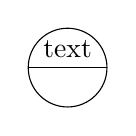
\begin{tikzpicture}
	\draw circle (0.5);
	\draw (-0.5, 0) to ["text"] (0.5, 0);
\end{tikzpicture}

\end{document}

